\section{Conversión de numero Binario a Decimal}

\subsection{Descripción del problema}

Dada una tabla de verdad de n bits generar la expresión booleana que genere de manera fidedigna las salidas de esta tabla. 

\subsection{Definición  de solución}

La solución a este problema implica identificar las operaciones lógicas (como AND, OR, NOT,) y las combinaciones adecuadas de las variables de entrada que permitan reproducir los resultados de la tabla de verdad en todas las combinaciones posibles de los valores de entrada.

\begin {figure}[h!]
\centerline{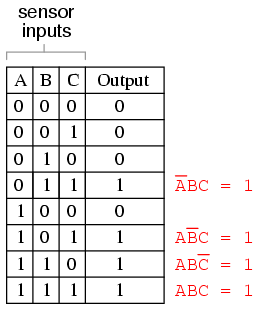
\includegraphics[width = 4cm]{imagen/booleanas.png}}
\caption{Binario a decimal.}
\label{fig}
\end {figure}

\subsection{Diseño de Solución}

Para poder codificar la  tabla de verdad  con n bits y la expresión booleana :

\begin{enumerate}
  \item Se crea un conjunto para almacenar las filas que el usuario desea cambiar.
  \item Se solicita al usuario el número de bits.
  \item Se inicia un bucle for que se imprimen los encabezados de las variables (A, B, C, etc.).
  \item Se imprime una fila de la tabla de verdad original y  el resultado, que es siempre 0 en la tabla original.
  \item  Se utiliza while para Bucle para Cambiar Bits y Se lee la fila que el usuario desea cambiar.
   Si el usuario ingresa 0, se sale del bucle.
  \item Se valida que la fila esté en el rango válido. Se vuelve al inicio del bucle si la fila no es válida.
  \item Se imprimen las expresiones booleanas asociadas a las filas modificadas. Se imprime la expresión booleana final.
  \item Se imprime cada bit de la fila en formato binario. Se imprime el resultado (1 o 0) de acuerdo a las filas cambiadas.
  \item Se genera la expresión booleana para una fila específica.
  \item Se genera la expresión booleana final concatenando las expresiones de las filas modificadas.
  
\end{enumerate}

\subsection{Desarrollo de Solución}


\begin{javaCode}
import java.util.Scanner;

public class Ejercicio_6_basico {
    public static void main(String[] args) {
        Scanner scanner = new Scanner(System.in);
        
        System.out.print("Ingrese el número de bits para la Tabla de Verdad: ");
        int numBits = scanner.nextInt();
        
        // Imprime encabezados de las variables
        for (int i = 0; i < numBits; i++) {
            System.out.print((char) ('A' + i) + "\t");
        }
        System.out.println("Resultado");
        
        // Inicializa la tabla de verdad con todos los resultados en 0
        int[] tablaVerdad = new int[(int) Math.pow(2, numBits)];
        
        // Imprime tabla de verdad original
        imprimirTabla(tablaVerdad, numBits);
        
        // Cambia las filas
        while (true) {
            System.out.print("Ingrese el número de la fila que desea cambiar a 1 (1-" + (int) Math.pow(2, numBits) + ") o ingrese 0 para finalizar: ");
            int fila = scanner.nextInt();
            
            if (fila == 0) {
                break;
            }
            
            if (fila < 1 || fila > Math.pow(2, numBits)) {
                System.out.println("Número de fila inválido. Debe estar entre 1 y " + (int) Math.pow(2, numBits) + ".");
                continue;
            }
            
            tablaVerdad[fila - 1] = 1;
            
            imprimirTabla(tablaVerdad, numBits);
        }
    }

    private static void imprimirTabla(int[] tablaVerdad, int numBits) {
        System.out.println("Tabla de verdad actualizada:");
        for (int i = 0; i < tablaVerdad.length; i++) {
            imprimirFilaTabla(i, numBits);
            System.out.println(tablaVerdad[i]);
        }
    }

    private static void imprimirFilaTabla(int valor, int numBits) {
        for (int j = numBits - 1; j >= 0; j--) {
            System.out.print(((valor >> j) & 1) + "\t");
        }
    }
}
\end{javaCode}

\subsection{Depuración y pruebas}

\begin {figure}[h!]
\centerline{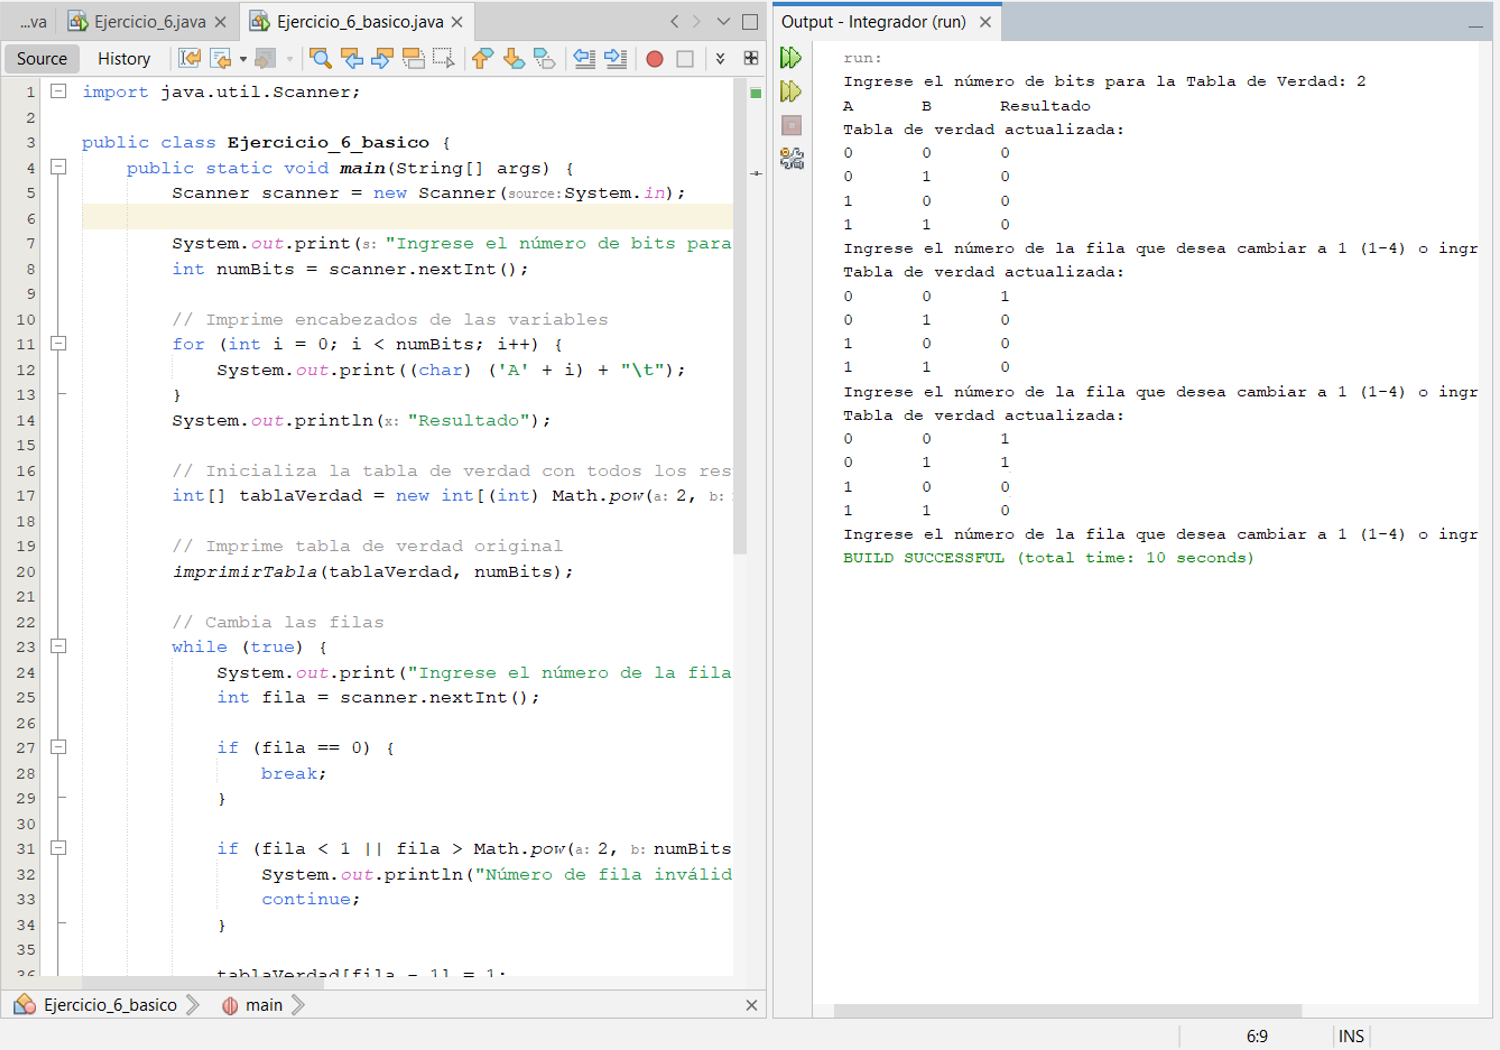
\includegraphics[width = 9.5cm]{imagen/tabla de verdad de 2 datos.png}}
\caption{Corrida 3}
\label{fig}
\end {figure}

\begin {figure}[h!]
\centerline{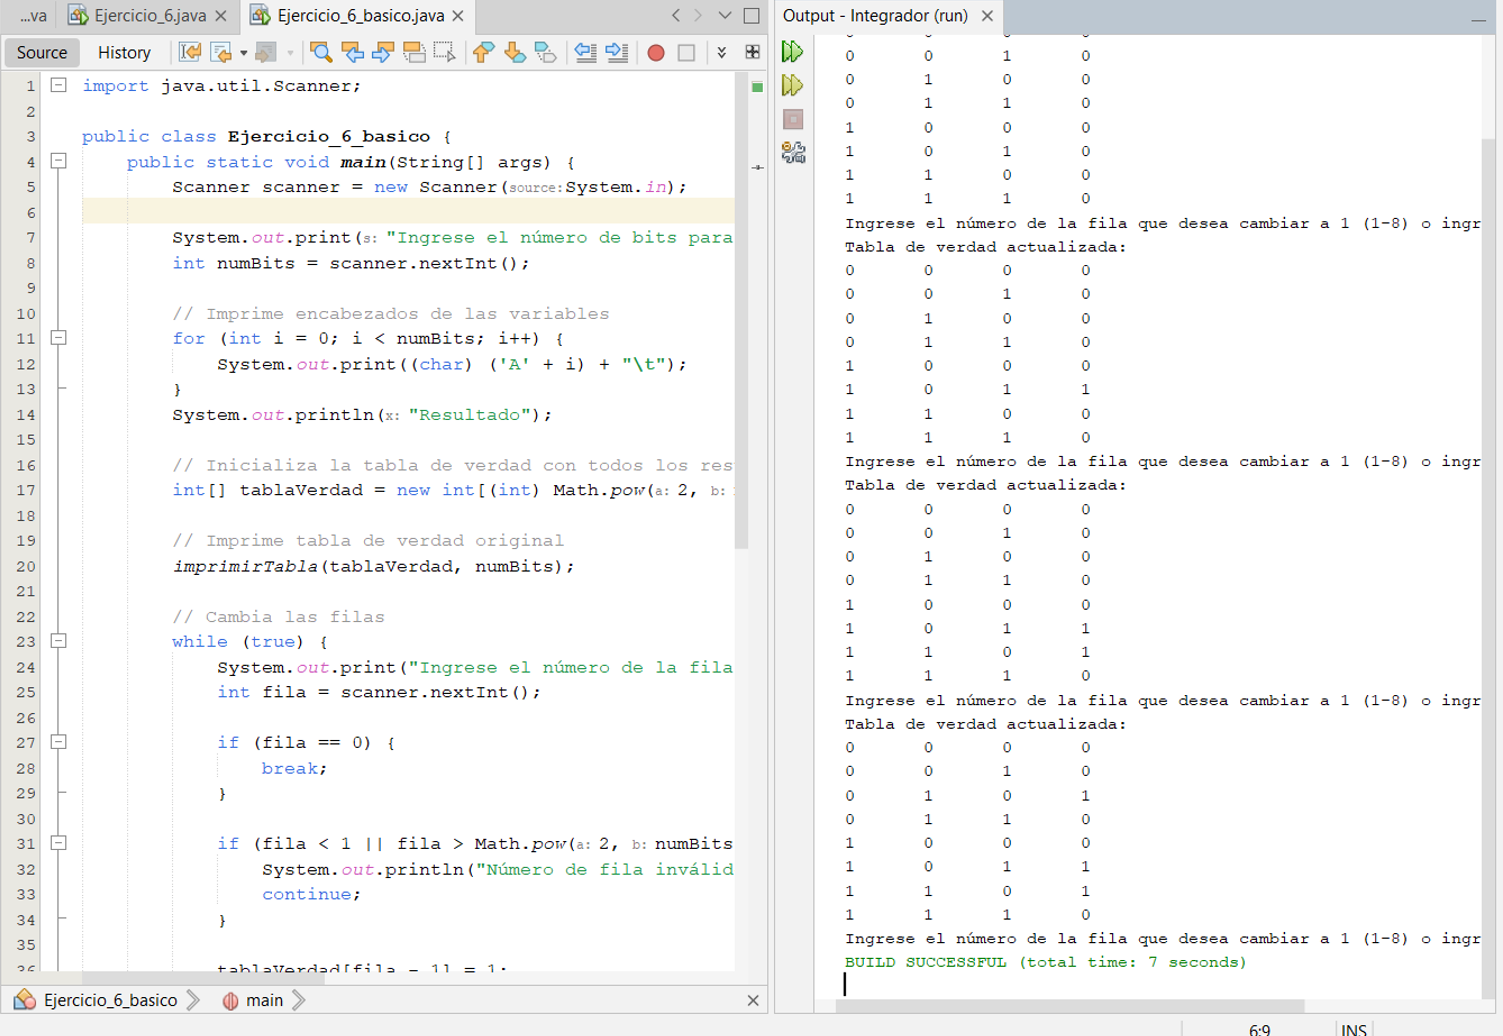
\includegraphics[width = 9.5cm]{imagen/tabla de verdad de 3 datos.png}}
\caption{Corrida 3}
\label{fig}
\end {figure}